\documentclass[autodetect-engine,dvipdfmx-if-dvi,ja=standard,everyparhook=compat]{bxjsarticle}

\usepackage{graphicx}        % 図を表示するのに必要
\usepackage{color}           % jpgなどを表示するのに必要
\usepackage{amsmath,amssymb} % 数学記号を出すのに必要
\usepackage{type1cm}         % fontsizeのエラー回避
\usepackage{here}            % 図の強制配置
\usepackage{url}             % URLをいい感じにしてくれる
\usepackage{subfigure}       % 図をまとめて表示
\usepackage{pdfpages}        % PDFの連結
\usepackage{setspace}
\usepackage{cases}
\usepackage{fancyhdr}
\usepackage{wrapfig}% 図の回り込み


% 余白の設定
% \setlength{\textheight}{\paperheight}   % 紙面縦幅を本文領域にする(BOTTOM=-TOP)
% \setlength{\topmargin}{-15.4truemm}     % 上の余白を10mm(=1inch-15.4mm)に
% \addtolength{\topmargin}{-\headheight}  %
% \addtolength{\topmargin}{-\headsep}     % ヘッダの分だけ本文領域を移動させる
% \addtolength{\textheight}{-20truemm}    % 下の余白も10mm
% \setlength{\textwidth}{\paperwidth}     % 紙面横幅を本文領域にする(RIGHT=-LEFT)
% \setlength{\oddsidemargin}{-5.4truemm}  % 奇数ページの左の余白を20mm(=1inch-5.4mm)に
% \setlength{\evensidemargin}{-5.4truemm} % 偶数数ページの左の余白を20mm(=1inch-5.4mm)に
% \addtolength{\textwidth}{-40truemm}     % 右の余白も20mm

% タイトル
\title{タイトル}

% ヘッダとフッタの設定
% \lhead{電気電子情報工学実験}
% \chead{}
% \rhead{20315784 佐藤凌雅}
% \lfoot{}
% \cfoot{\thepage} % ページ数
% \rfoot{}

\parindent = 0pt  % 行頭の字下げをしない
\setstretch{1.0}  % 行間

% キャプションの英語化
\renewcommand{\figurename}{Fig.}
\renewcommand{\tablename}{Table}

% 各章,節などタイトルの大きさを変更
% \titleformat*{\section}{\Huge\bfseries}
% \titleformat*{\subsection}{\Large\bfseries}

% 式の番号を(senction_num.num)のようにする
% \makeatletter
% \@addtoreset{equation}{chapter}
% \def\theequation{\thechapter.\arabic{equation}}
% \makeatother

% 呼び出したページのページ番号を消す
\newcommand{\deletePageNum}{
    \thispagestyle{empty}
    \clearpage
    \addtocounter{page}{-1}
}

% urlのフォントを直す
\renewcommand\UrlFont{\rmfamily}


\begin{document}
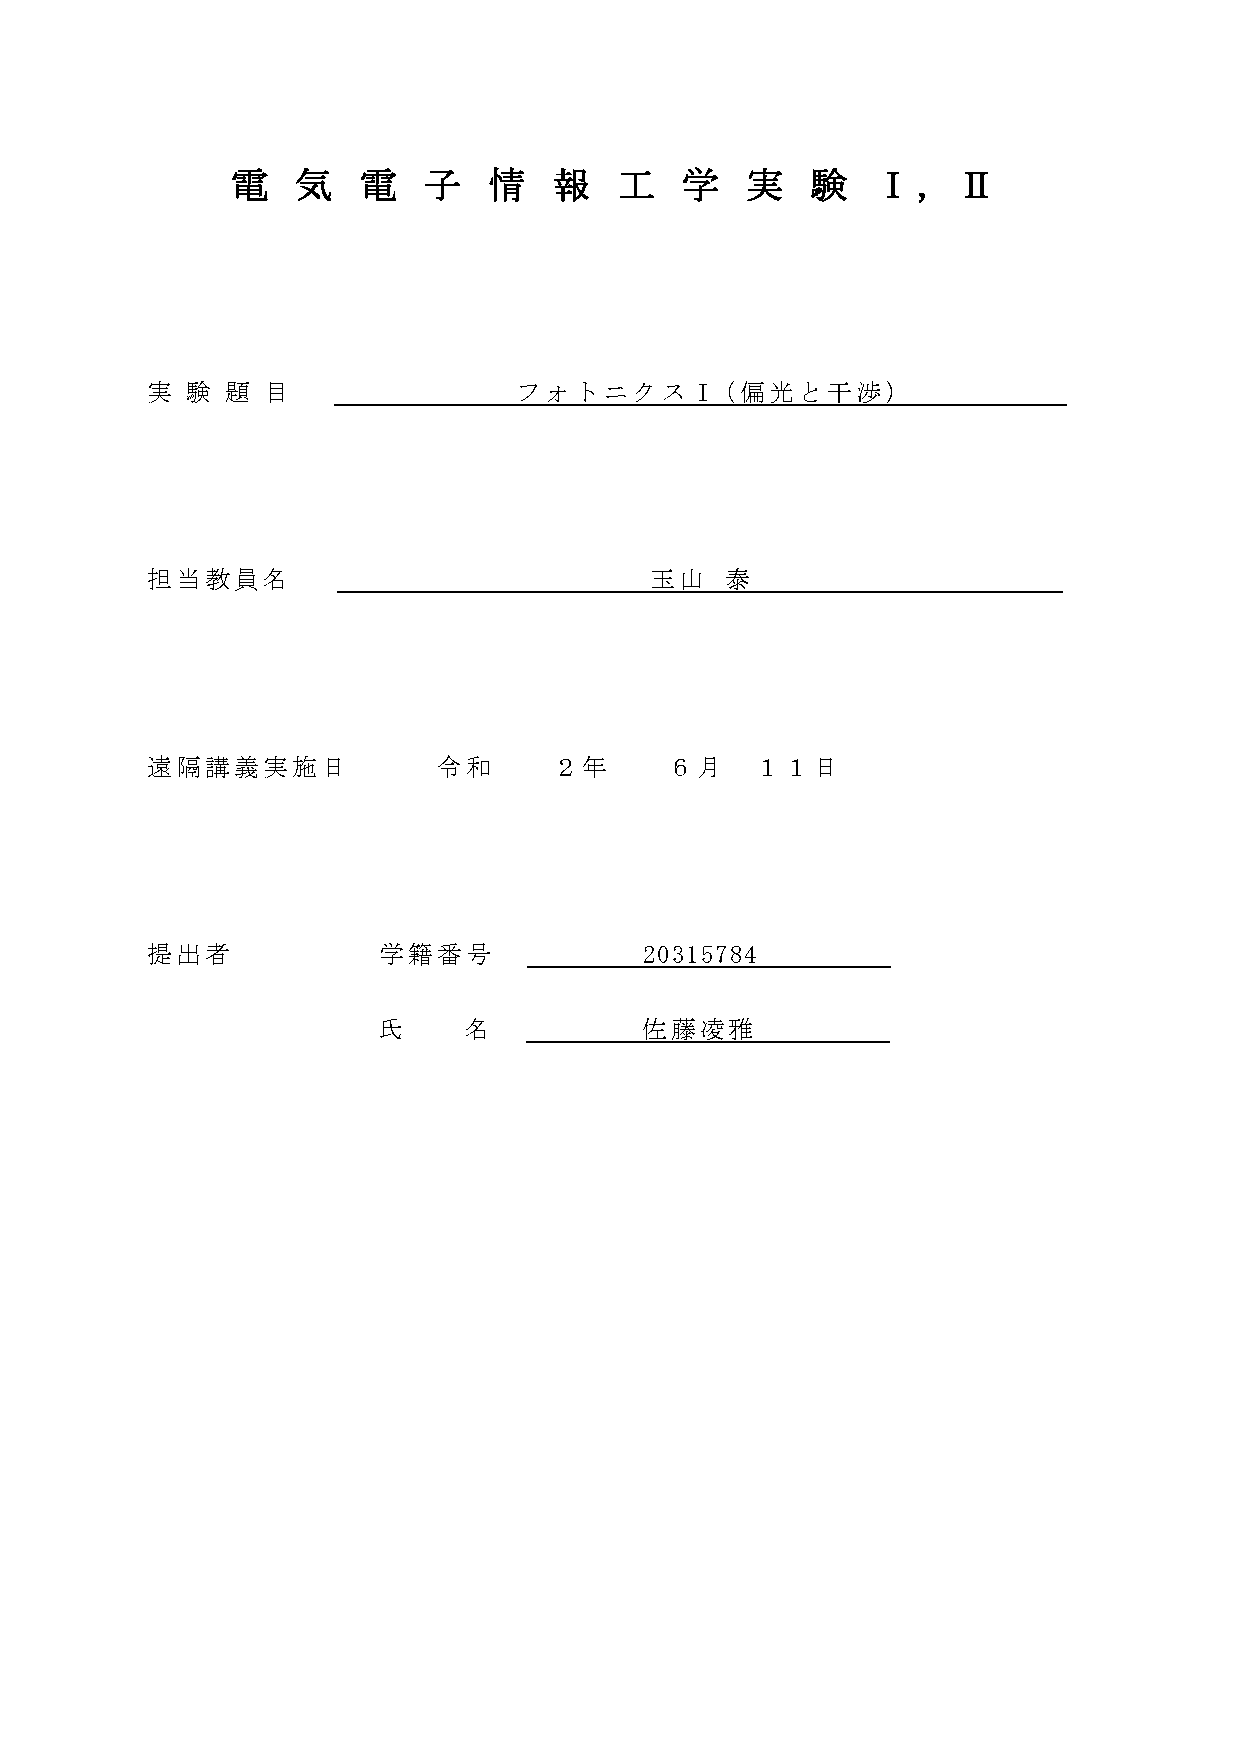
\includepdf[pages=-]{./setting/cover.pdf}
\fontsize{11.041pt}{16.562pt}\selectfont


% 実験の目的,手段,結果,結論を簡潔にまとめ示すこと.(250字程度)
% \section{概要 Abstract}


% テキストに書かれている目的等を参考に,各自どの点に注目して実験したのかを明確に示すこと.(300字程度)
\section{目的 Purpose}
 誘電体表面での光の反射に関する実験を通して,p偏光とs偏光の反射率特製の違いを調査する.\\
 ダブルスリットを使用した光の干渉実験を通して,干渉縞の出来方などから光の波動性を理解する.\\
 いずれの実験についても理論値と実測値との違いを比較,検討を行い,考察の過程で偏光と干渉について理解を深める.また,光学素子の扱いや光学実験手法についても学ぶ.さらに,グループ作業を通じて,限られた時間での効率的な作業方法などについても検討する.


% 各自の実験目的に必要な理論的な背景を示すこと.必要ならば,参考文献リストより文献番号を引用すること.(レポート用紙1枚程度)
\section{理論的背景 Theory}
\subsection{誘電体表面での光の反射}
 誘電体表面での光波の反射(フレネル反射)は、入射光の偏光に依存する.入射波,屈折波,反射波の電場ベクトルが入射面に対して平行である場合をp偏光,垂直である場合をs偏光と呼ぶ.この時,Fig.\ref{fig:refraction}に示すようにそれぞれの媒質の屈折率を$n_1$,$n_2$とすると,入射角を$\phi$と屈折角を$\chi$の間にはスネルの法則(Eqn.(\ref{eqn:Snell}))が成立する.
\begin{equation}
    \frac{\sin \phi}{\sin \chi} = \frac{n_2}{n_1}
    \label{eqn:Snell}
\end{equation}

\begin{figure}[H]
    \centering
    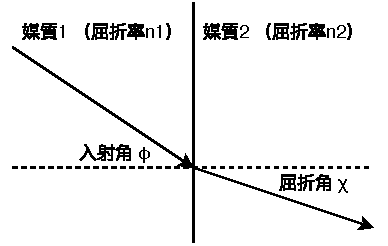
\includegraphics[width=6cm]{./fig/fig1.pdf}
    \caption{refraction}
    \label{fig:refraction}
\end{figure}

 また,p偏光,s偏光の反射率はEqn.(\ref{eqn:Fresnel_p})およびEqn.(\ref{eqn:Fresnel_s})で与えられる.
\begin{eqnarray}
    \left(R_{\mathrm{E}}\right)_{\mathrm{p}}&=&\frac{\tan ^{2}(\varphi-\chi)}{\tan ^{2}(\varphi+\chi)}
    \label{eqn:Fresnel_p} \\
    \left(R_{\mathrm{E}}\right)_{\mathrm{s}}&=&\frac{\sin ^{2}(\varphi-\chi)}{\sin ^{2}(\varphi+\chi)}
    \label{eqn:Fresnel_s}
\end{eqnarray}


 反射率について,p偏光の時には$\phi+\chi=\pi/2$の時に$\tan(\phi+\chi)\rightarrow\infty$となり,分母が発散するため,$R_E = 0$となる$\chi$が存在する.一方で,s偏光では分母が発散することはない.数式上,$\phi-\chi=0$の時に分子が0となるため,反射率が0になるように見えるが,スネルの法則より,入射角と反射角が同じになるのは$\phi = \pi/2$の時のみである.この時,Eqn.(\ref{eqn:Fresnel_s})は0/0の不定形となる.きちんと極限計算を行うと,$\phi = \pi/2$の時,反射率は1となるのでs偏光では反射率が0となることはない.\\

 前述のように,反射率が0となるのはp偏光の時のみである.p偏光の反射率が0となる時の入射角をブリュースター角と呼び,$\phi_B$で表す.先ほど示したように$R_E = 0$となるのは$\phi_B+\chi=\pi/2$,すなわち$\chi=\pi/2-\phi_B$の時であった.これをスネルの法則(Eqn.(\ref{eqn:Snell}))に代入して整理する.
\begin{equation}
    \frac{n_2}{n_1} = \frac{\sin \phi_B}{\sin \chi} = \frac{\sin \phi_B}{\sin (\pi/2-\phi_B)} = \frac{\sin \phi_B}{\cos \phi_B} = \tan \phi_B
\end{equation}

 この時,媒質1を空気であるとする($n_1 = 1$)と,ブリュースター角$\phi_B$はEqn.(\ref{eqn:Brewster})で表される.
\begin{equation}
    \phi_B = \tan^{-1} (n_2)
    \label{eqn:Brewster}
\end{equation}

\subsection{ダブルスリットを通過した光の干渉}
 Fig.\ref{fig:diagram_of_the_light_interference_experiment}のように,レーザー光を二つのスリットに対して一様に照射すると、それぞれのスリットから出射した光の干渉により,スクリーン上には明線と暗線が交互に現れる.スリットの中心間距離を$d$,ダブルスリットとスクリーンとの間の距離を$L$とする.この時,上側のスリットからスクリーン上の位置$x$までの距離$l_1$は三平方の定理よりEqn.(\ref{eqn:l1})となる.
\begin{figure}[H]
    \centering
    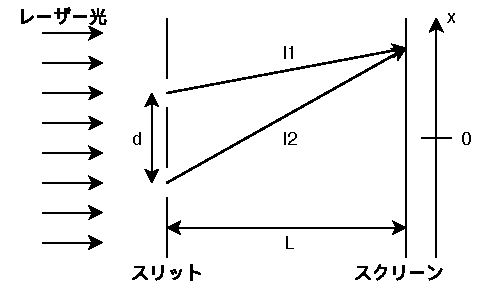
\includegraphics[width=7cm]{./fig/fig2.pdf}
    \caption{Diagram of the light interference experiment}
    \label{fig:diagram_of_the_light_interference_experiment}
\end{figure}

\begin{equation}
    l_1 = \sqrt{L^2+\left(x-\dfrac{d}{2}\right)^2} = L\sqrt{1+\left(\dfrac{x-\dfrac{d}{2}}{L}\right)^2}
    \label{eqn:l1}
\end{equation}

 ここで,一般化二項定理により$|α| << 1$の時に$\sqrt{1 + \alpha} \approx 1 + (1/2)\alpha$と近似できることが知られている. $L$は十分に大きいとすると$l_1$はEqn.(\ref{eqn:l1_approx})と近似できる.
\begin{equation}
    l_1 \approx L \left(1+\frac{1}{2}\left(\frac{x-\dfrac{d}{2}}{L}\right)^2\right) = L + \frac{1}{2L}\left(x-\frac{d}{2}\right)^2
    \label{eqn:l1_approx}
\end{equation}

同様にすると$l_2$はEqn.(\ref{eqn:l2_approx})となる.
\begin{equation}
    l_2 \approx  L + \frac{1}{2L}\left(x+\frac{d}{2}\right)^2
    \label{eqn:l2_approx}
\end{equation}

$l_1$と$l_2$の差は
\begin{eqnarray}
    l_2 - l_1 &=& L + \frac{1}{2L}\left(x+\frac{d}{2}\right)^2 - \left( L + \frac{1}{2L}\left(x-\frac{d}{2}\right)^2\right) \nonumber\\
    &=& \frac{1}{2L}\left(\left(x-\frac{d}{2}\right)^2-\left(x+\frac{d}{2}\right)^2\right) = \frac{1}{2L}(2dx) = \frac{d}{L}x
\end{eqnarray}

 距離に波数をかけると位相変化になるので,各スリットから出射した光のスクリーン上の位置$x$における位相差$\delta$は$\delta = kdx/L$となる.したがって,
\begin{equation}
    x = \frac{m \lambda L}{d}
\end{equation}
の時に光は強めあい,

\begin{equation}
    x = \dfrac{\left(m+\dfrac{1}{2}\right) \lambda L}{d}
\end{equation}
の時に光は打ち消しあう.

よって
\begin{eqnarray}
    \cos(\omega t) + \cos(\omega t - \delta) &=& 2\cos\left(\frac{2 \omega t - \delta}{2}\right)\cos\left(\frac{\omega t - \omega t - \delta}{2}\right) \nonumber\\
    &=& 2\cos\left(\frac{2 \omega t - \delta}{2}\right) \cos\left(\frac{\delta}{2}\right)
\end{eqnarray}

$\omega t$を除いた箇所が光強度に寄与しており,また,光強度は電界の振幅の二乗に比例するため,
\begin{eqnarray}
    I(x) &=& I_0 \left|  \cos\left(\frac{\delta}{2}\right) \right|^2 \nonumber\\
    &=& I_0 \left|  \cos\left(\dfrac{\dfrac{2 \pi d}{\lambda L}x}{2}\right) \right|^2 \nonumber\\
    &=& I_0 \left|  \cos\left(\dfrac{\pi d}{\lambda L}x\right) \right|^2
\end{eqnarray}

% 実験手段,測定系の概要,測定装置の名称・型番等を書くこと.また,装置の精度・仕様等の情報もできる限り示すこと.(レポート用紙2枚程度)
\section{実験方法 Experiment}
\subsection{誘電体表面での光の反射}
 p偏光およびs偏光のレーザー光をプリズムで反射させ,光検出器で検出を行う.レーザー光をp偏光またはs偏光へと変換するために,直線偏光子と$\lambda$/2板を用いる.また,入射角を容易に変化させられるよう,プリズムは回転ステージ上に取り付けられている.
\begin{figure}[H]
    \centering
    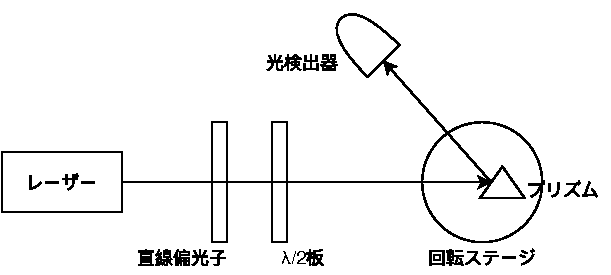
\includegraphics[width=7cm]{./fig/fig3.pdf}
    \caption{Diagram of the reflection experiment}
    \label{fig:diagram_of_the_reflection_experiment}
\end{figure}

\subsection{ダブルスリットを通過した光の干渉}
レーザー光をダブルスリットに対して一様に照射する.それぞれのスリットから出射した光の干渉により、スクリーン上には明線,暗線が交互に現れるので,光強度分布を観測する.
\begin{figure}[H]
    \centering
    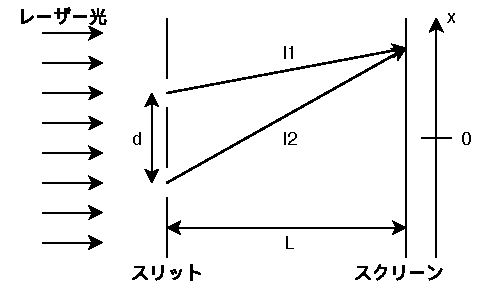
\includegraphics[width=7cm]{./fig/fig2.pdf}
    \caption{Diagram of the light interference experiment}
    \label{fig:diagram_of_the_light_interference_experiment}
\end{figure}

% % 各自の実験目的に沿った結果を簡潔にまとめること.その他の試行錯誤的実験データは Appendix にまとめる.枚数は各教員の指示に従ってください.(レポート用紙の枚数は教員の指示に従う)
% \section{実験結果 Results}

% % 各自の目的と照らし合わせ,測定結果の妥当性や数値計算結果との整合性などについて考察する.実験結果とサブテキスト/参考書の図式とを比較し議論すること.課題が与えられているテーマに関してはそれについても考察すること.(レポート用紙2枚程度)
% \section{考察 Discussion}

% % 君自身が実験を通じて(実験の方法,まとめ方などで)工夫した点をまとめる.(100字程度 )
% \section{工夫した点}

% 実験結果の羅列ではなく,考察した結果をまとめること.(250字程度)
% \section{まとめ Conclusion}

% レポートで引用した参考文献のリストを付ける.
% \section{参考文献 Reference}
% \begin{thebibliography}{9}
%     \bibitem{z80} 通信用語の基礎知識. Z80. \url{https://www.wdic.org/w/SCI/Z80}, (参照:2020-06-01)
%     \bibitem{assembly} IT用語辞典 e-Words. アセンブリ言語とは. \url{https://www.wdic.org/w/SCI/Z80}, (参照:2020-06-01)
% \end{thebibliography}


% % 周辺の関連調査事項,作成プログラムリスト,試行錯誤的実験データ
% \appendix
% \section{Appendix}

\end{document}
